\documentclass[9pt,twocolumn,twoside,lineno]{pnas-new}\usepackage[]{graphicx}\usepackage[]{xcolor}
% maxwidth is the original width if it is less than linewidth
% otherwise use linewidth (to make sure the graphics do not exceed the margin)
\makeatletter
\def\maxwidth{ %
  \ifdim\Gin@nat@width>\linewidth
    \linewidth
  \else
    \Gin@nat@width
  \fi
}
\makeatother

\definecolor{fgcolor}{rgb}{0.345, 0.345, 0.345}
\newcommand{\hlnum}[1]{\textcolor[rgb]{0.686,0.059,0.569}{#1}}%
\newcommand{\hlstr}[1]{\textcolor[rgb]{0.192,0.494,0.8}{#1}}%
\newcommand{\hlcom}[1]{\textcolor[rgb]{0.678,0.584,0.686}{\textit{#1}}}%
\newcommand{\hlopt}[1]{\textcolor[rgb]{0,0,0}{#1}}%
\newcommand{\hlstd}[1]{\textcolor[rgb]{0.345,0.345,0.345}{#1}}%
\newcommand{\hlkwa}[1]{\textcolor[rgb]{0.161,0.373,0.58}{\textbf{#1}}}%
\newcommand{\hlkwb}[1]{\textcolor[rgb]{0.69,0.353,0.396}{#1}}%
\newcommand{\hlkwc}[1]{\textcolor[rgb]{0.333,0.667,0.333}{#1}}%
\newcommand{\hlkwd}[1]{\textcolor[rgb]{0.737,0.353,0.396}{\textbf{#1}}}%
\let\hlipl\hlkwb

\usepackage{framed}
\makeatletter
\newenvironment{kframe}{%
 \def\at@end@of@kframe{}%
 \ifinner\ifhmode%
  \def\at@end@of@kframe{\end{minipage}}%
  \begin{minipage}{\columnwidth}%
 \fi\fi%
 \def\FrameCommand##1{\hskip\@totalleftmargin \hskip-\fboxsep
 \colorbox{shadecolor}{##1}\hskip-\fboxsep
     % There is no \\@totalrightmargin, so:
     \hskip-\linewidth \hskip-\@totalleftmargin \hskip\columnwidth}%
 \MakeFramed {\advance\hsize-\width
   \@totalleftmargin\z@ \linewidth\hsize
   \@setminipage}}%
 {\par\unskip\endMakeFramed%
 \at@end@of@kframe}
\makeatother

\definecolor{shadecolor}{rgb}{.97, .97, .97}
\definecolor{messagecolor}{rgb}{0, 0, 0}
\definecolor{warningcolor}{rgb}{1, 0, 1}
\definecolor{errorcolor}{rgb}{1, 0, 0}
\newenvironment{knitrout}{}{} % an empty environment to be redefined in TeX

\usepackage{alltt}
% Use the lineno option to display guide line numbers if required.

\newcommand{\tom}[2]{{\color{red}{#1}}\footnote{\textit{\color{red}{#2}}}}
\newcommand{\josh}[2]{{\color{blue}{#1}}\footnote{\textit{\color{blue}{#2}}}}

\templatetype{pnasresearcharticle} % Choose template 
% {pnasresearcharticle} = Template for a two-column research article
% {pnasmathematics} %= Template for a one-column mathematics article
% {pnasinvited} %= Template for a PNAS invited submission
\title{Context-dependent host-microbe interactions in stochastic environments}

% Use letters for affiliations, numbers to show equal authorship (if applicable) and to indicate the corresponding author
\author[a,1]{Joshua C. Fowler}
\author[b]{Shaun Ziegler}
\author[b]{Kenneth D. Whitney} 
\author[b]{Jennifer A. Rudgers}
\author[a]{Tom E. X. Miller}


\affil[a]{Rice University, Department of BioSciences, Houston, TX, 77005}
\affil[b]{University of New Mexico, Department of Biology, Albuquerque, NM, 87131}

% Please give the surname of the lead author for the running footer
\leadauthor{Fowler} 

% Please add here a significance statement to explain the relevance of your work
\significancestatement{Authors must submit a 120-word maximum statement about the significance of their research paper written at a level understandable to an undergraduate educated scientist outside their field of speciality. The primary goal of the Significance Statement is to explain the relevance of the work in broad context to a broad readership. The Significance Statement appears in the paper itself and is required for all research papers.}

% Please include corresponding author, author contribution and author declaration information
\authorcontributions{Please provide details of author contributions here.}
\authordeclaration{Please declare any conflict of interest here.}
\correspondingauthor{\textsuperscript{1}To whom correspondence should be addressed. E-mail: jcf3\@rice.edu}

% Keywords are not mandatory, but authors are strongly encouraged to provide them. If provided, please include two to five keywords, separated by the pipe symbol, e.g:
\keywords{Keyword 1 $|$ Keyword 2 $|$ Keyword 3 $|$ ...} 

\begin{abstract}
Microbial symbioses are ubiquitous in nature, yet our ability to predict how these interactions affect species' responses to climate change has been limited by interaction outcomes that vary with environmental context. Increased environmental variability is a key prediction of climate change. Here we present and test a novel hypothesis: microbial symbionts may buffer hosts from environmental variability by being beneficial in harsh years while being neutral or costly in good years. Long-term data reveal that, while weaker than effects on the mean of population growth, variance buffering is an important contribution to hosts long-term population growth. Additionally, the symbiosis becomes more mutualistic under simulated increases in variability, driven by an increased contribution from variance buffering.

Please provide an abstract of no more than 250 words in a single paragraph. Abstracts should explain to the general reader the major contributions of the article. References in the abstract must be cited in full within the abstract itself and cited in the text.
\end{abstract}

\dates{This manuscript was compiled on \today}
\doi{\url{www.pnas.org/cgi/doi/10.1073/pnas.XXXXXXXXXX}}
\IfFileExists{upquote.sty}{\usepackage{upquote}}{}
\begin{document}

\maketitle
\thispagestyle{firststyle}
\ifthenelse{\boolean{shortarticle}}{\ifthenelse{\boolean{singlecolumn}}{\abscontentformatted}{\abscontent}}{}

% If your first paragraph (i.e. with the \dropcap) contains a list environment (quote, quotation, theorem, definition, enumerate, itemize...), the line after the list may have some extra indentation. If this is the case, add \parshape=0 to the end of the list environment.
%Introduction
\dropcap{A}long with increases in average temperatures, global climate change is driving increases in the variability of precipitation events, temperature extremes, and droughts \cite{IPCC2012managing, seneviratne2012changes, stocker2013technical}. 
Discerning the effects of environmental variability on population dynamics and species interactions are therefore key objectives of global change ecology. 

\tom{}{It would be nice to start paragraph 2 here, but that probably leaves P1 too skimpy.}Classic theory predicts that long-term population growth rates (equivalently, population mean fitness) will decline under increased environmental variability due to negative effects of bad years that outweigh positive effects of good years (a consequence of nonlinear averaging) \cite{lewontin_population_1969,tuljapurkar_population_1982}. 
For example, in unstructured populations, the long-term stochastic growth rate in fluctuating environments ($\lambda_s$) will always be less than the growth rate averaged across environments ($\overline{\lambda}$) by an amount proportional to the environmental variance ($\sigma^2$): $ log(\lambda_s)  \approx log(\overline{\lambda}) - \frac{\sigma^2}{2\overline{\lambda}^2}$.
Populations structured by size or stage are expected to similarly experience negative effects of variability \cite{cohen1979comparative, tuljapurkar2013population}.
Thus, there are two pathways to increase population viability in a stochastic environment $\lambda_s$: increasing the mean growth rate and/or dampening temporal fluctuation in growth rates, also called variance ``buffering''.

Given the potential for negative fitness consequences of increasing environmental stochasticity under global change, there is growing interest in factors that can amplify or dampen demographic fluctuations. 
%\tom{That both mean and variance are important in determining fitness underlies understanding of which aspects of a species' life history influence its success \cite{pfister1998patterns, morris2008longevity} and has important implications for population viability analysis \cite{menges1990population}.}{I don't know what this sentence is saying.} 
Much attention has focused on the properties of species or their environment as modifiers of fluctuations in fitness, including variation in vital rates (survival, growth and reproduction)\cite{morris2008longevity}, correlations between vital rates \cite{compagnoni2016effect}, transient shifts in stage structure \cite{ellis2013role}, and the degree of environmental autocorrelation \cite{tuljapurkar1980population, fieberg2001stochastic}. 
In contrast, little is known about how biotic interactions influence patterns of demographic variability \cite{hilde_demographic_2020}, due in part to the paucity of long-term interaction data that are required to detect such effects.
%This pg needs work - what is the point of it? Also need transition sentence to microbes

Our work focused on the potential for microbial symbionts to buffer host plants against negative effects of environmental variability.
Microbial symbioses are ubiquitous across plant and animal host taxa and can be crucial determinants of host fitness \cite{rodriguez2009fungal, mcfall2013animals}.
Yet we know little about their potential influence on responses to climate change and environmental variation \cite{rudgers2020climate}. 
\tom{Across a broad range of taxa, mutualistic host-associated microbes provide protection from environmental stresses including drought, extreme temperatures, and enemies \cite{russell2006costs, brownlie2009symbiont, kivlin2013fungal,corbin2017heritable, hoadley2019host}.}{This sentence seems to contradict the previous sentence.} 
\tom{The role they play may be under-appreciated, and it can be difficult to quantify the net outcome of a given interaction because they are often viewed as being context-dependent where the magnitude of benefit depends on environmental conditions \cite{chamberlain2014context}. 
Rather than considering context-dependence as some unexplainable intricacy of species interactions, environmental variation opens up the possibility for interaction strength to vary through time \cite{jordano1994spatial, billick2003relative} and to influence the variance of population growth rates. }{I agree that this is the place to introduce context-dependence and connect climate variability to variability in interaction outcome. But I don't think what you have here works.}

\tom{We hypothesize that symbionts may provide benefits under harsh conditions when they are needed by their hosts, but be neutral or even costly under benign conditions. 
Over time, this would lead symbiotic hosts to experience a reduction in variation in vital rates by reducing the frequency of extreme years. 
Incorporating context-dependence in this way, we highlight a novel mechanism by which symbionts can act as mutualists that may come to be of increasing importance in a more variable future.}{Similar comment as above. I think this is the place to lay out the hypotheses of symbionts elevating mean and/or reducing variance. But I don't think this is sufficiently explanatory or provides sufficient context or rationale for the ideas to really hit home.}

Using data from a unique, long-term symbiont-removal experiment, we \tom{test the hypothesis that context-dependent benefits of microbial symbionts buffer hosts from the fitness consequences of environmental variability}{In addition to this hypothesis, I think it is important to emphasize the question of relative importance of mean vs variance effects. Like Volker always says, yes/no hypotheses are often a little dull.}. 
The experiment consists of annually censused plots initiated in 2007 with seven grass species that host Epichlo\"{e} fungal endophytes. 
These specialized fungal endophytes are unique to grasses, occurring in at least \tom{30\%}{I think the 30\% number comes from a Leuchtmann paper.} of cool-season (C3) species, and are primarily vertically transmitted from maternal plant to seed \cite{cheplick2009ecology}. 
\tom{While they have been associated with contributing to drought tolerance for their hosts}{Awkward phrasing.}, these \tom{benefits are commonly context-dependent}{This is a little confusing because it sounds like you are saying that the drought benefit is context-dependent, but I think drought is the context, so the benefits vary with presence or absence of drought.}\cite{cheplick2004recovery, kannadan2008endophyte, decunta2021systematic}. 
\tom{And so}{too colloquial}, we ask first how fungal endophytes influence the mean and interannual variance of their hosts' vital rates; next, we ask if these vital rate effects buffer variance in fitness and, if so, what is the relative contribution of variance buffering vs. mean effects to the overall effect of the symbiosis on long-term growth rates. 
\tom{To answer these questions, we build structured, stochastic population models for these seven grass host species (\textit{Agrostis perennans}, \textit{Elymus villosus}, \textit{Elymus virginicus}, \textit{Festuca subverticillata},\textit{Lolium arundinaceum}, \textit{Poa alsodes} and \textit{Poa sylvestris}).}{Mention the models somewhere in this paragraph but don't list the species. Species list should definitely go somewhere and should include the endophyte species to the best of our known -- maybe this is an appendix table.} 
\tom{These long-term plots contain either naturally symbiotic plants (E+) or those which have had their symbionts experimentally removed (E-).}{Should come earlier when you first introduce the ``unique'' experiment.}  
Each annual census is a sample of climatic variation. 
\tom{Across 14 years, the data contain 31,216 individual-transition years.}{Put in results.} 
After quantifying endophyte effects on mean and variance in population growth rates, we use simulations to explore the \tom{consequences of variance buffering under increased variance}{SHould be emphasized earlier. It's cool and novel.} \tom{and construct climate-explicit population models}{I would not mention this here since it is not central to the story of the paper.} to evaluate the role of climate drivers as explanations for this buffering. 

\tom{Intriguingly, we find that the symbiosis contributes positively to long-term population growth rates through both mean and variance buffering effects. Integrating across diverse effects on vital rates, contributions to long-term growth rates from effects on the mean are 4.17 times greater on average than contributions from variance buffering. However, these effects varied between species; for example, two species (\emph{A. perennans} and \emph{P. syvestris}) have contributions from variance buffering which are greater than mean effects. Additionally, the effect of mutualism increases under simulations with increased variance driven by greater contributions of variance buffering. In the most extreme scenario, we find that variance buffering contributions across species are 1.5 times greater than effects on the mean on average, and that variance buffering contributions are greater than mean effects for five out of seven species.}{I would eliminate this paragraph entirely. Not needed, since you launch directly into results from here.}

\section*{Results}
\begin{figure*}%[tbhp]
\centering
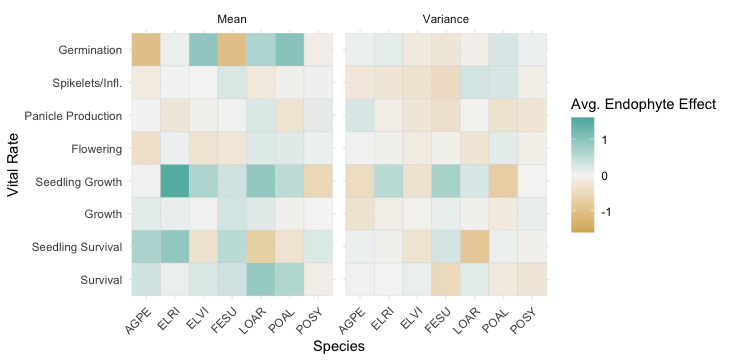
\includegraphics[width=.8\linewidth]{meanvar_effect_heatmap}
\caption{needs to be updated pdf version, but putting this here for now. Effect of endophytes on vital rates across species}
\label{fig:vr_figure}
\end{figure*}
\tom{}{I changed all your tenses to past tense.}
\subsection*{Endophyte effects on the mean and variance of vital rates}
Across eight host species, seven vital rates, 14 years, and \textit{large number} individual host-plants, we found that Epichlo\"{e} fungal endophyte symbiosis generally had positive effects on host demographic performance and negative effects on inter-annual demographic variance.
The mean endophyte effect was positive for \textit{number} out of $56$ host species--vital rate combinations, and was particularly strong for host survival and growth. 
Endophytes also consistently reduced inter-annual variance for the majority of host species and vital rates (\textit{number} out of $56$ host species--vital rate combinations; Fig. \ref{fig:vr_figure}), consistent with the hypothesis of variance buffering. 
Variance buffering effects were particularly strong for reproductive vital rates (e.g. likelihood of flowering and panicle production); \tom{This might align with predictions from life-history theory suggesting that reproductive vital rates are likely to experience greater year-to-year variance \cite{}.}{This is an interesting and possibly useful observation here, but it implies that negative effects on variance were proportional to the absolute value of variance. This seems plausible - is that the case? Also, the best citation would be Pfister 1998.} 

\tom{The}{We talked about updating the figure so that individual examples would pop out of the matrix. Presumably you would reference that figure here where you talk about specific examples.} relative magnitude of symbiont effects on means and variances was idiosyncratic across species and across vital rates. 
For example, endophytes increased mean adult survival and caused a modest variance reduction for \emph{P. alsodes}, while for \emph{F. subverticillata}, effects from variance buffering were stronger with a relatively weaker mean effect. 
In other vital rates, such as in seedling growth, \emph{P. alsodes} experiences stronger buffering than \emph{F. subverticillata}. 
\josh{Interestingly, there were also certain vital rates that showed \tom{costs}{If you are going to highlight costs then it would be good to show both reductions in mean and increases in variance.} of endophyte symbiosis, such as \emph{A. perennans} and \emph{F. subverticillata} which had lower mean germination rates when partnered with endophytes.}{Not sure how much to talk about demographic compensation (i.e. do we see less variance in vital rates that are more important). We don't really assess this. And at least loooking at the actual sigma values for each species, it seems like none of the vital rates have hugely different baseline standard deviations. TOM: I would not talk about demographic compensation.} 

\subsection*{Endophyte effects on the mean and variance of population growth rates}
Not all vital rates contribute equally to fitness, so we used stochastic matrix models (where tiller number was the integer-valued state variable) to integrate the diverse effects described above into comprehensive measures for the mean and variance of host fitness.
We found that, on average across host species, endophyte-symbiotic populations experienced a 9.2 \% increase in mean fitness $\overline{\lambda}$. 
Our hierarchical Bayseian analysis, which propagates uncertainty from the underlying data through model predictions, indicates 92.8\% confidence that endophytes increased $\overline{\lambda}$.
The \tom{standard deviation}{The figure in this draft shows CV. We should be consistent with what is shown and described.}, reflecting inter-annual variability in fitness, was 6.6 \% lower in endophyte-symbiotic populations than endophyte-free populations, averaging across host species (with \tom{66\% certainty}{The CV figure I am looking at is more than 66\% certainty.} that the endophyte effect was negative) (Fig. \ref{fig:lambda_figure}). 
\tom{For some host species, the standard deviation was  reduced by as much as 44.3\% (\emph{L. arundinaceum}) and 28.5\% (\emph{F. subverticillata}), while for others, variance effects were much smaller, or even slightly positive (\emph{E. villosus} and \emph{E. virginicus}).}{I am thinking it might be valuable to show that biplot}{Here is where I think the biplot figure makes an interesting point. For some species the benefit is through the mean, for some it is through variance, for some it is both -- but we don't see any negative-negative. It's really compelling evidence for mutualism being pervasive here, but taking different forms.}
\tom{}{This comment is neither here nor there, but we can probably expct reviewers to ask was the realized population growth patterns were, i.e., did E+ plots grow faster than E- plots. Not sure how much we should go there yet (because the populations mostly shrank) but I do think we need to better communicate that we are talking about asymptotic growth rates.}

\begin{figure*}%[tbhp]
\centering
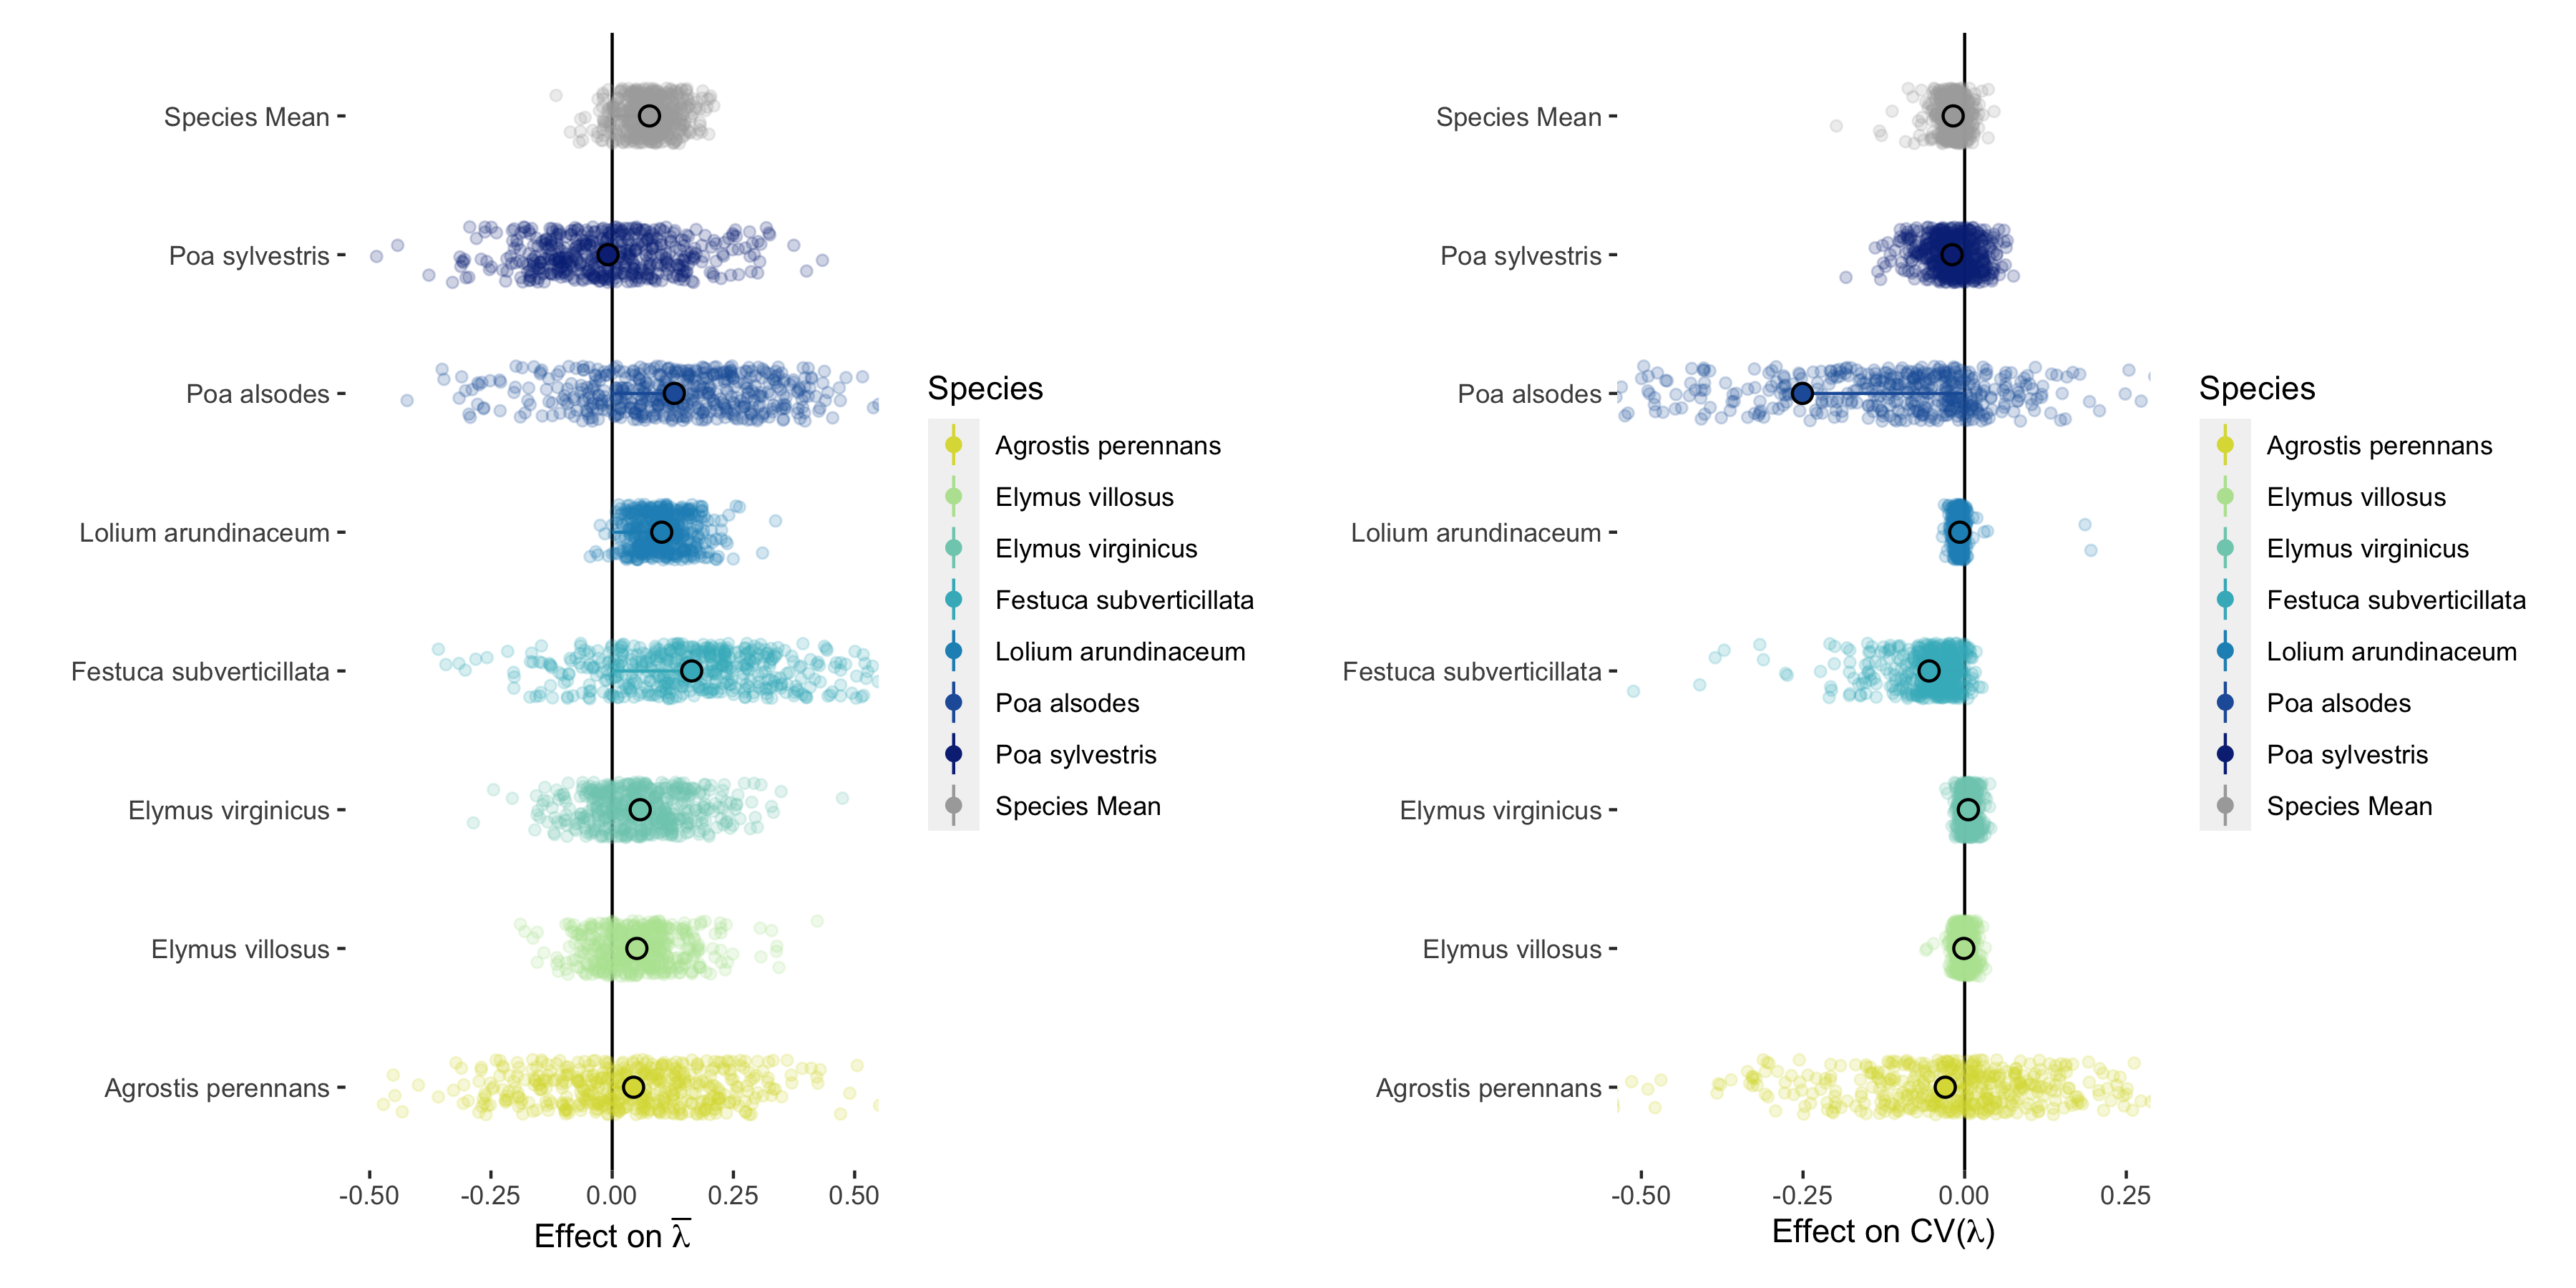
\includegraphics[width=.8\linewidth]{endo_lambdaeffects_plot}
\caption{needs to be updated pdf version, but putting this here for now. Effect of endophytes on mean and CV of population growth}
\label{fig:lambda_figure}
\end{figure*}

\subsection*{Contribution of mean and variance effects to long-term growth rates}
Having documented positive fitness effects of endophyte symbiosis via mean benefits and / or variance buffering, we next asked about the relative importance of those two pathways of host-symbiont mutualism for the stochastic growth rate $\lambda_{S}$.
We decomposed the overall effect of the symbiosis on $\lambda_{S}$ into contributions from mean and variance buffering effects  \josh{\citep{rees2009integral}}{I don't know if there's a better citation for this, this is more about IPM's-- Tom: I don't think we need a citation here, but we should briefly describe how we did this, since readers will get here before the methods. I've tried to add a little of this throughout the Results.}. 
\tom{We found that variance buffering provided a small benefit overall (XXX\%)}{Seems like this section is still under construction, but be sure to emphasize that across species there is really strong evidence for mutualism (positive effect on $\lambda_{S}$) and in the current regime of environmental variability that is dominated by the mean benefits.} (Fig. \ref{fig:contributions_plot}) \tom{but note that even small changes in fitness can have profound effects over long time periods}{probably would not say this}.

\begin{figure*}%[tbhp]
\centering
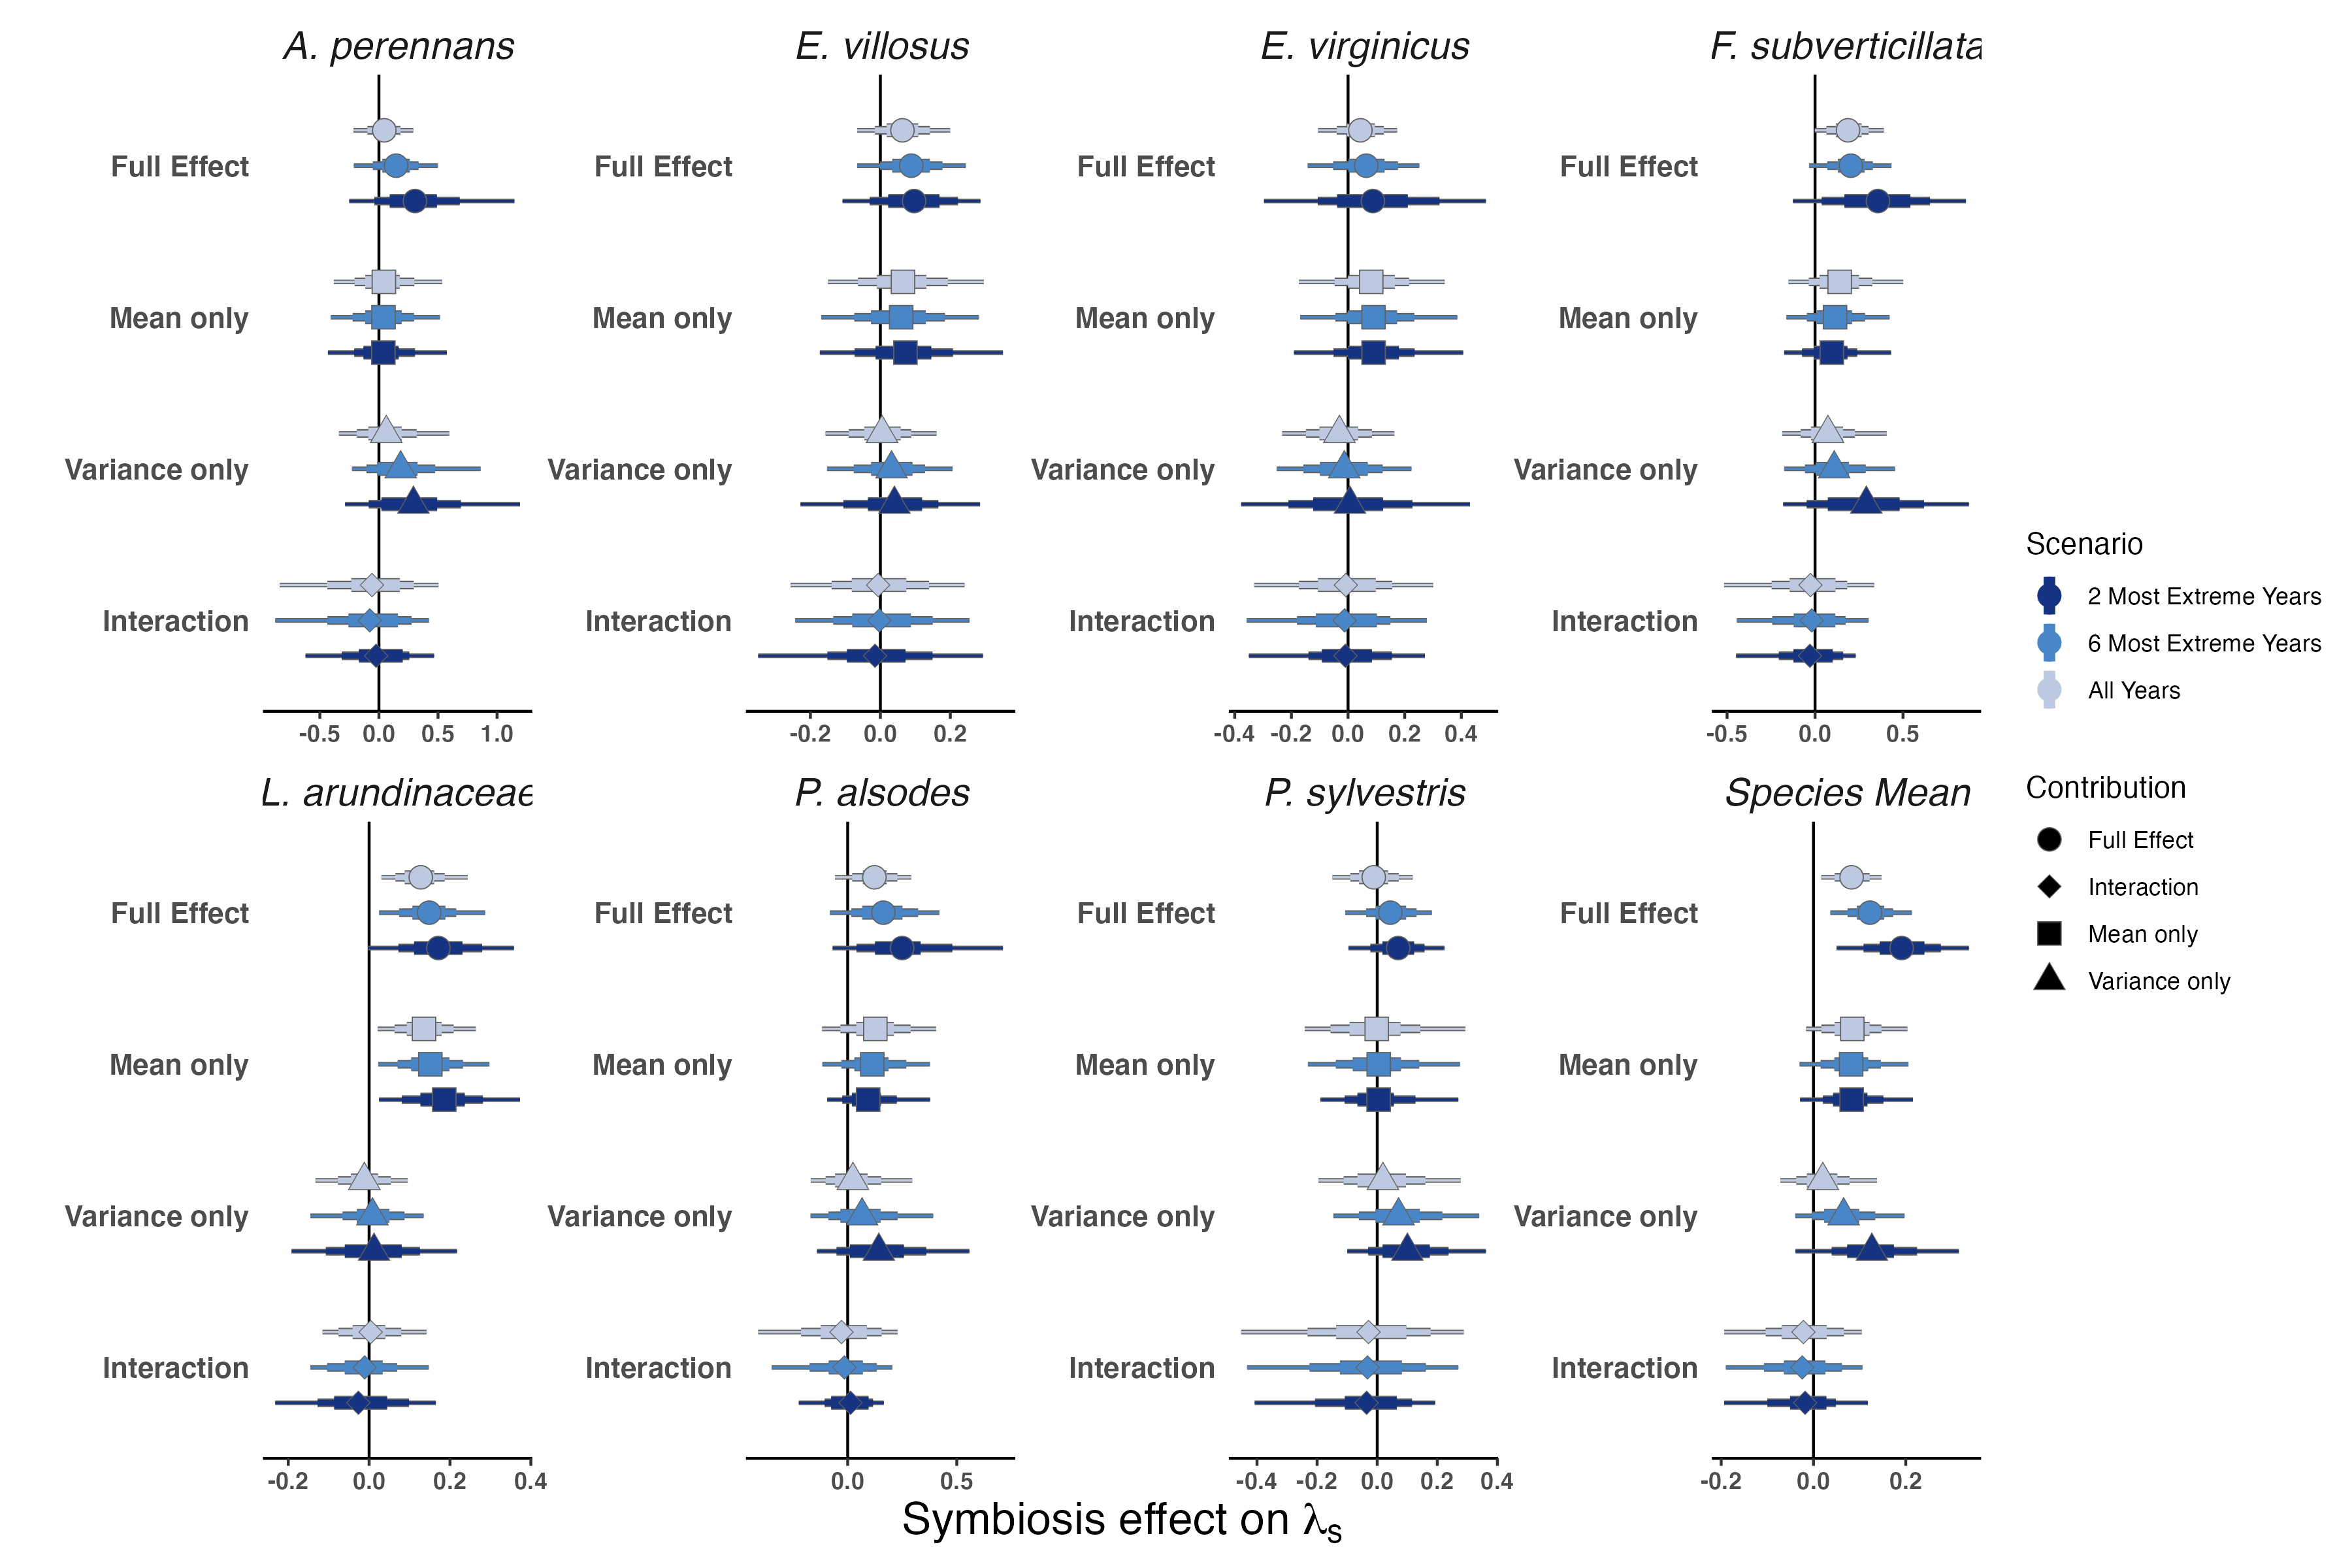
\includegraphics[width=.8\linewidth]{contributions_obs_plot}
\caption{needs to be updated pdf version, but putting this here for now. Stochastic lambda contributions with simulations of increased variance}
\label{fig:contributions_plot}
\end{figure*}


\subsection*{Role of symbiotic buffering under increased variance}

\tom{In simulations with increased variance, we find that the cnotribution of variance buffering increases.}{Skipping this for now, but it might make more sense to talk about the ambient and increased variance scenarios in the same results section, since they are in the same figure.}


\subsection*{Endophytes are buffering their hosts from environmental variability}
\tom{Symbiotic and non-symbiotic populations responded distinctly to environmental drivers. Our cllmiate-explicit analysis shows that on average, the population growth of non-endophytic plants was more sensitive to our drought index, SPEI, than endophytic populations (FIGURE). This pattern was particularly pronunced for species which showed strong buffering in our earlier analysis (SPECIES), suggesting that endophytes are buffering their hosts from this aspect of inter-annual variation, although a large amount of variation remained unexplained.}{I am wondering if it might be better to incorporate this material into the ealier section that describes variance buffering, so really what we are doing here is just providing a more mechanistic explanation for that phenomenological result.}


\section*{Discussion}

\section*{Guide to using this template on Overleaf}

Please note that whilst this template provides a preview of the typeset manuscript for submission, to help in this preparation, it will not necessarily be the final publication layout. For more detailed information please see the \href{http://www.pnas.org/site/authors/format.xhtml}{PNAS Information for Authors}.

If you have a question while using this template on Overleaf, please use the help menu (``?'') on the top bar to search for \href{https://www.overleaf.com/help}{help and tutorials}. You can also \href{https://www.overleaf.com/contact}{contact the Overleaf support team} at any time with specific questions about your manuscript or feedback on the template.

\subsection*{Author Affiliations}

Include department, institution, and complete address, with the ZIP/postal code, for each author. Use lower case letters to match authors with institutions, as shown in the example. Authors with an ORCID ID may supply this information at submission.

\subsection*{Submitting Manuscripts}

All authors must submit their articles at \href{http://www.pnascentral.org/cgi-bin/main.plex}{PNAScentral}. If you are using Overleaf to write your article, you can use the ``Submit to PNAS'' option in the top bar of the editor window. 

\subsection*{Format}

Many authors find it useful to organize their manuscripts with the following order of sections;  Title, Author Affiliation, Keywords, Abstract, Significance Statement, Results, Discussion, Materials and methods, Acknowledgments, and References. Other orders and headings are permitted.

\subsection*{Manuscript Length}

PNAS generally uses a two-column format averaging 67 characters, including spaces, per line. The maximum length of a Direct Submission research article is six pages and a Direct Submission Plus research article is ten pages including all text, spaces, and the number of characters displaced by figures, tables, and equations.  When submitting tables, figures, and/or equations in addition to text, keep the text for your manuscript under 39,000 characters (including spaces) for Direct Submissions and 72,000 characters (including spaces) for Direct Submission Plus.

\subsection*{References}

References should be cited in numerical order as they appear in text; this will be done automatically via bibtex, e.g. . All references should be included in the main manuscript file.  

\subsection*{Data Archival}

PNAS must be able to archive the data essential to a published article. Where such archiving is not possible, deposition of data in public databases, such as GenBank, ArrayExpress, Protein Data Bank, Unidata, and others outlined in the Information for Authors, is acceptable.

\subsection*{Language-Editing Services}
Prior to submission, authors who believe their manuscripts would benefit from professional editing are encouraged to use a language-editing service (see list at www.pnas.org/site/authors/language-editing.xhtml). PNAS does not take responsibility for or endorse these services, and their use has no bearing on acceptance of a manuscript for publication. 


\subsection*{Digital Figures}

Only TIFF, EPS, and high-resolution PDF for Mac or PC are allowed for figures that will appear in the main text, and images must be final size. Authors may submit U3D or PRC files for 3D images; these must be accompanied by 2D representations in TIFF, EPS, or high-resolution PDF format.  Color images must be in RGB (red, green, blue) mode. Include the font files for any text. 

Figures and Tables should be labelled and referenced in the standard way using the \verb|\label{}| and \verb|\ref{}| commands.

Figure \ref{} shows an example of how to insert a column-wide figure. To insert a figure wider than one column, please use the \verb|\begin{figure*}...\end{figure*}| environment. Figures wider than one column should be sized to 11.4 cm or 17.8 cm wide. Use \verb|\begin{SCfigure*}...\end{SCfigure*}| for a wide figure with side captions.

\subsection*{Tables}
In addition to including your tables within this manuscript file, PNAS requires that each table be uploaded to the submission separately as a Table file.  Please ensure that each table .tex file contains a preamble, the \verb|\begin{document}| command, and the \verb|\end{document}| command. This is necessary so that the submission system can convert each file to PDF.

\subsection*{Single column equations}

Authors may use 1- or 2-column equations in their article, according to their preference.

To allow an equation to span both columns, use the \verb|\begin{figure*}...\end{figure*}| environment mentioned above for figures.

Note that the use of the \verb|widetext| environment for equations is not recommended, and should not be used. 

\begin{figure*}[bt!]
\begin{align*}
(x+y)^3&=(x+y)(x+y)^2\\
       &=(x+y)(x^2+2xy+y^2) \numberthis \label{eqn:example} \\
       &=x^3+3x^2y+3xy^3+x^3. 
\end{align*}
\end{figure*}


\begin{table}%[tbhp]
\centering
\caption{Comparison of the fitted potential energy surfaces and ab initio benchmark electronic energy calculations}
\begin{tabular}{lrrr}
Species & CBS & CV & G3 \\
\midrule
1. Acetaldehyde & 0.0 & 0.0 & 0.0 \\
2. Vinyl alcohol & 9.1 & 9.6 & 13.5 \\
3. Hydroxyethylidene & 50.8 & 51.2 & 54.0\\
\bottomrule
\end{tabular}

\addtabletext{nomenclature for the TSs refers to the numbered species in the table.}
\end{table}

\subsection*{Supporting Information (SI)}

Authors should submit SI as a single separate PDF file, combining all text, figures, tables, movie legends, and SI references.  PNAS will publish SI uncomposed, as the authors have provided it.  Additional details can be found here: \href{http://www.pnas.org/page/authors/journal-policies}{policy on SI}.  For SI formatting instructions click \href{https://www.pnascentral.org/cgi-bin/main.plex?form_type=display_auth_si_instructions}{here}.  The PNAS Overleaf SI template can be found \href{https://www.overleaf.com/latex/templates/pnas-template-for-supplementary-information/wqfsfqwyjtsd}{here}.  Refer to the SI Appendix in the manuscript at an appropriate point in the text. Number supporting figures and tables starting with S1, S2, etc.

Authors who place detailed materials and methods in an SI Appendix must provide sufficient detail in the main text methods to enable a reader to follow the logic of the procedures and results and also must reference the SI methods. If a paper is fundamentally a study of a new method or technique, then the methods must be described completely in the main text.

\subsubsection*{SI Datasets} 

Supply Excel (.xls), RTF, or PDF files. This file type will be published in raw format and will not be edited or composed.


\subsubsection*{SI Movies}

Supply Audio Video Interleave (avi), Quicktime (mov), Windows Media (wmv), animated GIF (gif), or MPEG files and submit a brief legend for each movie in a Word or RTF file. All movies should be submitted at the desired reproduction size and length. Movies should be no more than 10 MB in size.


\subsubsection*{3D Figures}

Supply a composable U3D or PRC file so that it may be edited and composed. Authors may submit a PDF file but please note it will be published in raw format and will not be edited or composed.


\matmethods{
\subsection*{Natural history of grass-endophyte symbiosis}
\tom{To}{I think much of this info should go at the end of the Intro -- although as a natural history section I think this is lacking.} study the effects of context-dependent microbial symbiosis, we focused on \emph{Epichloë} fungal endophytes, which live in the aboveground tissue of many species of cool-season grasses and grow into their hosts' seeds where they can be transmitted vertically from mother to offspring plants. 
\tom{This vertical transmission couples host and symbiont fitness and leads to the expectation that the interaction be mutualistic, else the fungi cause their host to be selected out of the population \citep{fine1975vectors, douglas1998host, rudgers2009fungus}.}{This is not natural history, it is theory.} 
While there are demonstrated benefits against herbivory\citep{brem2001epichloe} and under drought stress \citep{hamilton2012new} for some host species, \tom{these interactions outcomes are commonly context-dependent}{The ``while'' structure of this sentence confuses me, because benefits against drought and herbivory \textbf{is} context-dependence.} \citep{cheplick2004recovery, kannadan2008endophyte}.\tom{}{This is in fact very little natural history in this paragraph, which I think is a problem. You've said little about endophytes and nothing about hosts.}

\subsection*{Plant propagation and endophyte removal}
Seeds from naturally \tom{infected}{Be strategic and consistent in your language for E+. I would not say ``infected''.} populations of seven species of cool-season grasses (\emph{Agrostis perennans}, \emph{Elymus villosus}, \emph{Elymus virginicus}, \emph{Festuca subverticillata}, \emph{Lolium arundinaceum}, \emph{Poa alsodes}, and \emph{Poa sylvestris}) were collected during the 2006 growing season from Lilly Dickie Woods (39.238533, -86.218150) and the Bayles Road Teaching and Research Preserve (39.220167, -86.542683) in Brown County, Indiana, USA. 
\tom{To reduce confounding genotype effects, seeds with shared maternal ancestry}{Wording here makes it hard to follow the main point: that E- amd E+ seeds share the same maternal genetic background. I think that can be stated more directly.} were disinfected with heat treatments \tom{(6d in a drying oven at 60$^{\circ}$ C for \emph{E. villosus}, \emph{E. virginicus}, \emph{F. subverticillata},  and \emph{L. arundinaceum}; 7d in a drying oven at 60$^{\circ}$ C for \emph{P. alsodes}, and \emph{P. sylvestris}; and 12 min. in a hot water bath at 60$^{\circ}$ C for \emph{A. perennans})}{need to double check methods for temp, duration, etc.} or left naturally infected. 
Seeds were surface sterilized with bleach and cold stratified for {\color{red}??? weeks}, then germinated in a growth chamber before being transferred to the greenhouse at Indiana University and allowed to grow for XXXX weeks. 
We confirmed the endophyte status of these plants using microscopy of leaf peels, where tissue from the leaf sheath is stained with aniline blue and examined for the presence of fungal hyphae \citep{bacon2018stains}. 
Then, we established the experimental plots with \tom{vegetatively propogated clones of similar sizes from the plants}{not sure this happened} to reduce the potential for \tom{negative side effects}{Should explain how this reduces negative side effects.} of heat treatments \cite{rudgers2009benefits}.

\subsection*{Experimental design and data collection}
During the spring of 2007, we established 10 3x3 plots for \emph{A. perennans}, \emph{E. villosus}, \emph{E. virginicus}, \emph{F. subverticillata}, and \emph{L. arundinaceum}  and \tom{18 plots for \emph{P. alsodes} and \emph{P. sylvestris}}{I think one set was started in 2007 and another in 2008.}. 
For each species, five (or nine, for \emph{P. alsodes} and \emph{P. sylvestris}) plots were randomly assigned to each endophyte status, \tom{E+ or E-}{I don't think you have used this notation consistently. We will need to tighten this up.}. 
Each plot was planted with 20 evenly spaced \tom{symbiotic or symbiont-free}{Example of previous comment.} individuals and each plant received a unique aluminum tag staked into the ground. 

Each summer starting in 2007 and through 2021, we censused all individuals in each plot for survival, growth and reproduction, generating a data set covering 14 years that contains 31,216 \tom{individual transition years}{YOu have not defined or described this and I doubt most readers will understand what you mean. I think it's better to describe data collection first, introduce the idea of an individual transition as fllowing on plant from t to t+1, then give the sample size. This number does not make sense yet because you have not said that we added recruits to the census.}. 
Leaf litter was cleared out of each plot prior to the census, to aid in locating all tagged individuals and new recruits.
For each plant alive in the previous year, we marked its survival, measured its size as a count of the number of tillers, and collected reproductive data by counting the number of reproductive tillers, and then counting the number of seed-bearing spikelets on up to three of those reproductive tillers. 
In 2009, we took additional counts of seeds per inflorescence. 
%Together, we use these measurements to estimate seed production. 
\tom{In each plot, we also search for and tag any unmarked individuals, which are recruits from previous years' seed production.}{Say this earlier.} 
\tom{New recruits typically have one tiller and are non-reproductive, but we also find and tag any individuals that may have been missed in previous censuses.}{Not necessary, but say we collect the same data on recruit and original plants.}

We typically expect plots of each endophyte status to maintain their status because the fungi are almost entirely vertically transmitted and plots are {\color{red}spaced at least 5 m apart}, limiting the possibility of dispersal between plots or \tom{horizontal transmission of the symbiont}{We have data on choke symptoms, right? I think we should quantify and report this. We also have data showing that plots mostly stayed true to endo status, and we should include this too.}. 
Seeds from reproductive individuals are opportunistically taken and \tom{scored}{scored how} for their endophyte status. 
Overall, these scores reflect a \tom{97.5\%  faithfulness of recruits}{This is better than I recall - we should check.} to their expected endophyte status across species and plots (Supplement data).

\subsection*{Demographic modeling}
\tom{}{Up to you but I think it will make more sense to start with the statistical models, then build to the matrix model -- which is the true order of operations and the order of results in the paper.}
\tom{Armed}{Word choice. Equipped?} with this demographic data, we next constructed size-structured, stochastic matrix projection models. 
These models describe transitions between sizes (measured as a count of tillers, a discrete state variable) from one year to the next. 
For all species, we include a 1 year reproductive delay in the population model following the observation that these \tom{newly recruited plants are rarely observed flowering in their first year}{I think we need to explain this further. It's not only that recruits do not reproduce. More importantly, their size alone does not identify them as a recruit, so we need an additional state variable.}. 
Our \tom{population model}{You are showing a deterministic model -- needs to be stochastic (A is time-varying.) But actually I recommend presenting this differently, more like what I did in the appendix of Iler et al (shared on slack). What you have here is not wrong but it invites the impression that we built the matrix model by building data, while we actually built it from vital rate regressions.} can be expressed as:

\begin{equation}
\label{eq:matrixmodel}
\mathbf{n}_{t+1} = \mathbf{A}\mathbf{n}_{t}
\end{equation}

where $\mathbf{n}_{t+1}$ is a vector of abundances across sizes in year t+1 for each species and endophyte status.

\begin{equation}
\label{eq:nvector}
\mathbf{n}_{t+1} = \begin{bmatrix} size^{sdlg} \\ size_{i} \\ . \\ .\\ . \\ size_{N} \end{bmatrix} 
\end{equation}

and $\mathbf{A}$ is expressed as a N+1 x N+1 matrix:
\begin{equation}
\label{eq:Amatrix}
\mathbf{A} = \begin{bmatrix} 0 & F_{i}  & . & . & F_{N} \\
                            T^{sdlg} & T_{i}  & . & . & .\\
                            . & .  & . & . & .\\
                            . & .  & . & . & .\\
                            T^{sdlg} & .  & . & . & T_{N} \end{bmatrix}
\end{equation}

in which \tom{$T$ and $F$ are size-transition (i.e. survival and growth)}{Again, not wrong, but one of the issues here is that there are lower-level parameters not represented here. Your $T$ is growth conditioned on survival. My suggestion, as in the Iler et al model, is the present the stat models first then use the same notation in the MPM.} and reproduction kernels drawn from our vital rate estimates for each species and endophyte status.


\subsubsection*{Statistical analysis of vital rates}
We modeled the effect of endophyte symbiosis on the mean and variance of vital rates by fitting generalized linear mixed models (GLMM) to the long-term data with year and plot random effects. 
We fit all vital rate models in a hierarchical Bayesian framework using Rstan \citep{Stan2022}, allowing us to isolate multiple sources of variance, borrow strength across species for some variance components, and propagate uncertainty from the vital rate estimates to our population model \citep{elderd2016quantifying}. 

The probabilities of survival and flowering \tom{are}{Flagging tense issues again. I would use past tense for methods.} \tom{recorded as successes or failures}{This sentence is incorrect as written: the probabilities were not recorded as success or failure.} and consequently are modeled as Bernoulli processes. 
We modeled growth (measured as the number of tillers in year $t+1$ conditions on number of tillers in year $t$) and the number of flowering tillers with a zero-truncated Poisson-Inverse Gaussian distribution, and the number of spikelets per inflorescence with the negative binomial distribution. 
Each of these size-dependent vital rates are modeled with the same structure of linear predictor ($\mu$)

\tom{For example,}{Since you are only showing growth and survival here, not sure this is necessary. I would show all of them or none of them (meaning just show linear predictor $mu$). } growth ($G_{i,t1})$ of a given \tom{individual (i) in year t+1}{I think there are some notation issues here. Let's work out the models on a white board.} is modeled as:
\begin{equation} 
\label{eq:growth}
\begin{aligned}
G_{i,t1} \sim P(IG(\mu_{s,e},\lambda_{s,e} )) \\
\end{aligned}
\end{equation}

Similarly, survival {$S_{i,t1}$} in year t+1 is modeled as:
\begin{equation} 
\label{eq:survival}
\begin{aligned}
S_{i,t1} \sim Bernoulli(\mu_{s,e}) \\
\end{aligned}
\end{equation}

Where $\mu$, for each species (s), is a linear function of the logarithm of plant size in year t (t), the plot-level endophyte status (e), whether the plant was part of the initial transplanting or naturally recruited into the plot (r), along with random effects to account for plot(p) and \tom{year variation specific to each species and endophyte status}{This is buried here but is probably the most important part of the entire project -- needs to really pop out and be explained clearly.}. 
Thus $\mu$ can be written:
\begin{equation}
\label{eq:linearpredictor}
\begin{aligned}
\mu_{s,e} = \beta^1_{s} + \beta^2_{s}log(size_{t}) + \beta^3_{s,e} + \beta^4_{r} \\
+  \tau + \rho \\
\tau \sim N(0,\sigma_{s,e}) \\
\rho \sim N(0,\sigma_{p})
\end{aligned}
\end{equation}
\tom{}{I think you need to explain that plot variance was shared across species.}
For all species, we account for a reproductive delay by modeling seedling growth and survival separately from adult growth and survival. 
Seedlings are those plants that are recruited into the plot in a given year, and typically have only one tiller. 
So, for seedlings, growth ($G^{sdlg}_{1,t1}$) is modelled as:

\begin{equation} 
\label{eq:sdlg_growth}
\begin{aligned}
G^{sdlg}_{1,t1} \sim P(IG(\mu^{sdlg}_{s,e},\lambda_{s,e} )) \\
\end{aligned}
\end{equation}

Similarly, survival ($S^{sdlg}_{i,t1}$) in year t+1 is modeled as:
\begin{equation} 
\label{eq:sdlg_survival}
\begin{aligned}
S^{sdlg}_{1,t1} \sim Bernoulli(\mu^{sdlg}_{s,e}) \\
\end{aligned}
\end{equation}

Here, $\mu^{sdlg}_{s,e}$ is the linear function for these seedling specific vital rates. 
It does not include size-dependence or a greenhouse rearing effect. 

\begin{equation}
\label{eq:sdlg_linearpredictor}
\begin{aligned}
\mu^{sdlg}_{s,e} = \beta^1_{s} + \beta^3_{s,e} \\
+ \tau + \rho \\
\tau \sim N(0,\sigma_{s,e}) \\
\rho \sim N(0,\sigma_{p})
\end{aligned}
\end{equation}

\tom{The final element}{For the sake of intuitive chronology, it might make more sense to describe the recruitment model before seedling growth and survival.} of the life cycle comes from recruitment of new plants from seeds produced the preceding year. 
For this, we modeled the probability of recruitment as a proportion of seeds produced from the \tom{preceding year}{We should be explicit here that we assume there is no seed bank.} with a \tom{Binomial regression}{Issues here: the binomial has two parameters, p and N. The N is the number of seeds produced the preceding year, which I believe you dervived from other vital rate models. This should be represented symbolically.}. 
\begin{equation} 
\label{eq:recruitment}
\begin{aligned}
R_{1,t1} \sim Binomial(\mu^{sdlg}_{s,e}) \\
\end{aligned}
\end{equation}

\begin{equation}
\label{eq:recruitment_linearpredictor}
\begin{aligned}
\mu^{rec}_{s,e} = \beta^1_{s} + \beta^3_{s,e} \\
+ \tau + \rho \\
\tau \sim N(0,\sigma_{s,e}) \\
\rho \sim N(0,\sigma_{p})
\end{aligned}
\end{equation}

We ran each vital rate model for 2500 warm-up and \tom{2500 MCMC sampling iterations}{Hmm, this is not very many, particularly for a nasty distribution like the PIG.} with three chains using rStan. 
We assessed model convergence with trace plots of posterior chains and checked for $\hat{R}$ values less than 1.01, indicating low within- and between-chain variation \citep{brooks1998general,gelman2006data}. 
For those models that showed poor convergence, we \tom{extended the MCMC sampling}{OK maybe 2500 was usually adequate.} to include 5000 warm-up and 5000 sampling iterations, which was only necessary for seedling growth. 
For each of these vital rate models, we graphically check model fit with posterior predictive checks comparing simulated data from 500 posterior draws with the observed data \tom{(See supplement?)}{Yes, put in appendix. Can reference those here.}. 
%These checks provide evidence that our models are accurately recreating size-specific growth, survival, and reproduction patterns in our data across endophyte treatments.

We calculate the effect of endophytes on mean and variance in population growth rates by assembling matrix models with and without endophyte symbiosis following equation [\ref{eq:matrixmodel}]. 
To do this, we calculated annual population growth rates for symbiotic and non-symbiotic populations for the 13 observed transition years by adjusting our vital rate estimates according to the year random effects, incorporating model uncertainty by sampling 500 posterior draws from our vital rate models. 
\tom{By using observed years, we maintain the structure of vital rate correlations as observed in the field.}{There is probably a good citation here, maybe Doak and Morris.} 
We then calculated the mean and \tom{variance}{Or Sd or CV?} of these annual growth rates. 

\subsection*{Stochastic growth rate simulation experiment}
We \tom{decomposed}{Before dwscribing any decomposition, I would start by saying that you calculated the stochastic growth rate, and say how.} the contribution of endophyte symbiosis to long-term stochastic growth rates by calculating the geometric mean of \tom{500 randomly sampled annual population growth rates}{Unclear if these are sampled years, or posterior samples based on the observation years.}, for simulated populations including \tom{mean-only, variance-only, and mean and variance endophyte effects compared to those without endophyte effects}{This needs a much more thorough explanation - very skimpy description of what was done and why.} {\color{red}\cite{tuljapurkar1980population}.can add better citations for this}\tom{}{Not sure but check Aldo's demographic correlations paper.}

\begin{equation}
\label{eq:stoch_sim}
\begin{aligned}
log(\lambda_s) = E[log(\Sigma(\mathbf{n}_{t+1})/\Sigma(\mathbf{n}_{t}))]
\end{aligned}
\end{equation}

To explore the potential effects of future increased climate variability, we calculated the stochastic growth rates as above for simulations which sample the most extreme observed years more frequently. 
\tom{To do this, we randomly sampled the six annual population growth rates that were furthest from the mean growth rate across E+ and E- populations.}{This is not what is shown in the figure.} 
\tom{Additionally, we tested the influence of temporal autocorrelation by sampling either alternating }{Did you do this?}

\subsection*{Estimating climate drivers of environmental context-dependence}
To ask \tom{whether the variance buffering effects of symbiosis are driven by environmental variation}{By definition, variance buffering effects must be driven by environmental variation.}, and to \tom{forecast population dynamics under future climate change scenarios}{Not really what we are doing here.}, we built climate-explicit population models. 
These models are built from vital rates as described above with the inclusion of a parameter describing the effect, for each endophyte status and species, of 12-month \tom{SPEI}{Spell out first time.}, a drought index that incorporates precipitation and evapotranspiration \cite{}.
 We calculated SPEI with weather station data from Bloomington, IN via the `rnoaa' and \cite{} `spei' R packages \cite{}. 
 This weather station has the most complete climate record over the study period and the historic record when compared to other nearby weather stations and \tom{is comparable to downscaled climate data}{Why say this?} (could include correlations) (See Supplement?). 
 \tom{Preliminary model selection}{Sounds wishy-washy.} using the climwin package \cite{} with simpler vital rate models suggested that a \tom{12-month SPEI}{I thought you compared 12 month to some other window.} would reasonably capture the relevant climate signal (see appendix?).
\subsubsection*{Forecasting under alternative climate forcings}
We performed model experiments to explore the effect of altered mean and variance in climate as expected under cilmate change. First, we generated a 50 year climate time series by randomly drawing observed SPEI values, 
\tom{}{This was probably written long ago and no longer relevant.}
}


\showmatmethods{} % Display the Materials and Methods section

\acknow{Please include your acknowledgments here, set in a single paragraph. Please do not include any acknowledgments in the Supporting Information, or anywhere else in the manuscript.}

\showacknow{} % Display the acknowledgments section

% Bibliography
\bibliography{endo_stoch_demo.bib}

\end{document}
